

\section{Introduction}

	\paragraph{Disentangling parameters' impact}
	Perovskite synthesis is a very easy and fragile process at the same time. When varying a fabrication parameter, for example during an optimization, it is quite likely to provoke a "butterfly effect" with the resulting device differing from the reference by much more than the characteristic under study.
	A principal component analysis of the fabrication parameters would be needed for a rational optimization, but such a complex procedure is further hindered by the difficulty of identifying all relevant contributions.

	\paragraph{Varying the thickness}
	In this study we vary a set of parameters that hopefully have a foreseeable relation with the resulting device structure: thickness of each layer, through the tuning of the spin coating deposition speed.
	The effect of this variation should just affect the layers thicknesses, having just a minor influence on the other device physical features.
	This will allow us to univocally relate the observations to the modifications.
%	each layer thickness variation to the characterization results variation.
	The complete devices were studied by means of current-voltage sweeps, \acr{ce}, \acr{tpv}, and \acr{dc}.

	\paragraph{The devices}
	The chosen architecture was an all-organic, solution processed, top cathode, two step perovskite deposition \gls{ito}\-/\gls{pedotpss}\-/\gls{mapi}\-/\gls{pcbm70}\-/\ch{Ag} device (fabrication described in \cpagerefrange{methods_top}{methods_top_end}).
	The layers whose thickness was independently varied are the \gls{pedotpss} (\gls{htm}), the \gls{mapi} (absorber), and the \gls{pcbm70} (\gls{etm}).
All these layers were deposited by spin coating and the thickness was tuned via spin coating speed as described in \cpagerefrange{methods_top}{methods_top_end}.
The champion device performances of each configuration are listed in \cref{table:thicknesses_jv}.


%\begin{table}%[h]	% longtables cannot stay inside a float, otherwise they will not break
\begin{xltabular}[c]{1\linewidth}{@{}>{\hsize=1.2\hsize}Y|>{\hsize=0.9\hsize}Y|>{\hsize=0.9\hsize}Y | c >{\hsize=1.5\hsize}Y >{\hsize=0.9\hsize}Y >{\hsize=0.8\hsize}Y >{\hsize=0.8\hsize}Y @{}}
	% multirow does not get the correct number of rows with tabularx
	% mycaption does not work inside xltabular
	\caption[Layers thicknesses and related average performances of top cathode cells.]{\textbf{Layers thicknesses and related average performances of top cathode cells.}
				Explored thicknesses with relative average forward and reverse J-V sweep performances.
				For each reported result, at least 8, 8, and 4 devices were averaged respectively for \gls{mapi}, \gls{pcbm70}, and \gls{pedotpss} thickness exploration.
				\Gls{etm} column indicates the \gls{pcbm70} thickness, while \gls{htm} one refers to \gls{pedotpss} thickness.
				The standard deviation for each value is indicated after the $\pm$ symbol.
				A boxplot representation of this data can be found in \authoryear{Gelmetti2017}.
				J-V curve for record devices are reported in \cref{fig:jv_champions-mapi,fig:jv_champions-pcbm,fig:jv_champions-pedotpss}.
			}\label{table:thicknesses_jv}\\[\belowcaptionskip]
\multicolumn3{c|}{\small\textbf{Layers thickness}} & \multicolumn{5}{c}{\small\textbf{J-V sweep parameters}}
\rule[-1ex]{0pt}{3ex} \\
	 \gls{mapi} &  \gls{etm} & \gls{htm} & Sweep & \gls{jsc} &  \gls{voc} & \gls{ff} &  \gls{pce} \\ 
	 \rule[-1ex]{0pt}{2.5ex}  \footnotesize$[\si{\nm}]$ &  \footnotesize$[\si{\nm}]$ &  \footnotesize$[\si{\nm}]$ & - & \footnotesize[\si{\mA\per\square\cm}] &  \footnotesize$[\si{\V}]$ & \footnotesize$[\si{\%}]$ &  \footnotesize$[\si{\%}]$ \\[1mm]
	\hline
	\endfirsthead
	\multicolumn{2}{@{}l}{\ldots \small continues}\\
	 \hline
	 \gls{mapi} & \gls{etm} & \gls{htm} & Sweep & \gls{jsc} & \gls{voc} & \gls{ff} & \gls{pce} \\ 
	\hline
	\endhead
	\hline
	\multicolumn{8}{r@{}}{\small continues\ldots}\\
	\endfoot
	\hline
	\endlastfoot
\rule[-1ex]{0pt}{3ex}
\multirow{3}{*}{230} 	& \multirow{11}{*}{40}	&  \multirow{11}{*}{65}	&fwd	&	13.5	$\pm	0.5	$ & 	1.03	$\pm	0.01	$ & 	53	$\pm	3	$ & 	7.3	$\pm	0.4	$ \\*
\rule[-1ex]{0pt}{2.5ex}
  						&  						& 						&rev	&	13.6	$\pm	0.5	$ & 	1.02	$\pm	0.01	$ & 	55	$\pm	3	$ & 	7.7	$\pm	0.5	$ \\*
\cline{1-1} \cline{4-8}
\multirow{3}{*}{320}	&  						&  						&fwd	&	13.9	$\pm	0.3	$ & 	1.04	$\pm	0.01	$ & 	57	$\pm	5	$ & 	8.2	$\pm	0.6	$ \\*
\rule[-1ex]{0pt}{2.5ex}
  						&  						&  						&rev	&	14.1	$\pm	0.3	$ & 	1.04	$\pm	0.01	$ & 	55	$\pm	4	$ & 	8.1	$\pm	0.5	$ \\*
\cline{1-1} \cline{4-8}
\multirow{3}{*}{440}	&  						&  						&fwd	&	16.3	$\pm	2.1	$ & 	1.01	$\pm	0.04	$ & 	58	$\pm	2	$ & 	9.5	$\pm	0.8	$ \\*
\rule[-1ex]{0pt}{2.5ex}
 						&  						&  						&rev	&	16.5	$\pm	1.9	$ & 	0.98	$\pm	0.07	$ & 	50	$\pm	5	$ & 	8.1	$\pm	1.4	$ \\[1mm]
\hline
\multirow{15}{*}{350}	& \multirow{3}{*}{40} 	&  \multirow{15}{*}{65} &fwd	&	16.4	$\pm	2.2	$ & 	0.93	$\pm	0.06	$ & 	48	$\pm	8	$ & 	7.4	$\pm	1.8	$ \\*
  						&  						&  						&rev	&	16.1	$\pm	2.1	$ & 	0.95	$\pm	0.06	$ & 	50	$\pm	5	$ & 	7.6	$\pm	1.4	$ \\*
\cline{2-2} \cline{4-8}
  						& \multirow{3}{*}{60} 	& 					 	&fwd	&	13.2	$\pm	1.1	$ & 	0.99	$\pm	0.04	$ & 	47	$\pm	6	$ & 	6.2	$\pm	1.1	$ \\*
	 					&  						&  						&rev	&	12.8	$\pm	0.7	$ & 	0.98	$\pm	0.05	$ & 	47	$\pm	5	$ & 	5.9	$\pm	0.8	$ \\*
\cline{2-2} \cline{4-8}
	  					& \multirow{3}{*}{90} 	&  						&fwd	&	11.1	$\pm	0.6	$ & 	1.03	$\pm	0.03	$ & 	42	$\pm	2	$ & 	4.8	$\pm	0.6	$ \\*
	  					&  						&  						&rev	&	11.1	$\pm	0.8	$ & 	1.00	$\pm	0.04	$ & 	44	$\pm	2	$ & 	4.8	$\pm	0.5	$ \\*
\cline{2-2} \cline{4-8}
  						& \multirow{3}{*}{120} 	&  						&fwd	&	7.7	$\pm	1.6	$ & 	1.02	$\pm	0.04	$ & 	18	$\pm	2	$ & 	1.4	$\pm	0.4	$ \\*
	  					&  						&  						&rev	&	7.6	$\pm	1.6	$ & 	1.01	$\pm	0.04	$ & 	18	$\pm	2	$ & 	1.4	$\pm	0.4	$ \\[1mm]
\hline
\multirow{11}{*}{300}	& \multirow{11}{*}{40}	& \multirow{3}{*}{27} 	&fwd	&	12.3	$\pm	1.5	$ & 	1.04	$\pm	0.03	$ & 	55	$\pm	9	$ & 	6.9	$\pm	0.8	$ \\*
  						&  						&  						&rev	&	11.9	$\pm	1.7	$ & 	1.03	$\pm	0.04	$ & 	54	$\pm	11	$ & 	6.6	$\pm	0.7	$ \\*
\cline{3-8}
  						&  						& \multirow{3}{*}{45} 	&fwd	&	12.2	$\pm	1.7	$ & 	1.04	$\pm	0.01	$ & 	58	$\pm	4	$ & 	7.3	$\pm	1.2	$ \\*
				  		&  						&  						&rev	&	11.8	$\pm	1.7	$ & 	1.00	$\pm	0.09	$ & 	53	$\pm	7	$ & 	6.2	$\pm	0.9	$ \\*
\cline{3-8}
				  		& 				 		& \multirow{3}{*}{65} 	&fwd	&	12.4	$\pm	1.6	$ & 	1.04	$\pm	0.02	$ & 	60	$\pm	3	$ & 	7.7	$\pm	0.6	$ \\*
				  		&  						&  						&rev	&	12.6	$\pm	1.4	$ & 	1.00	$\pm	0.10	$ & 	60	$\pm	4	$ & 	7.5	$\pm	0.4	$ \\[1mm]
\end{xltabular}




\section{Interpretation of \glsentryshort{jsc} and \glsentryshort{ff} from Current-Voltage Sweeps}

\section{Interpretation of Transient PhotoVoltage Referenced to Differential Capacitance}\label{interpretation_tpvdc}

\section{Varying \glsentrytext{mapi} Thickness (Absorber Layer)}

Using different spin coating speeds, devices with various \gls{mapi} thicknesses were obtained, as detailed in \cref{table:mapi_thickness}.
As a consequence to the different deposition conditions, the \gls{mapi} surface is more rough for the thick device than for the thin one, as can be intuited looking at \cref{fig:thickness-esem-topview}.
Any way, measuring the roughness average with a profilometer, it resulted to be \SI{< 10}{\nm} for all the cases, so that there's no doubt that the \SI{40}{\nm} \gls{pcbm70} layer is enough for ensuring a complete coverage.



\begin{figure}
	\makebox[\textwidth][c]{
		\parbox{1.1\textwidth}{
			\centering
			\begin{subfigure}[t]{0.51\textwidth}
				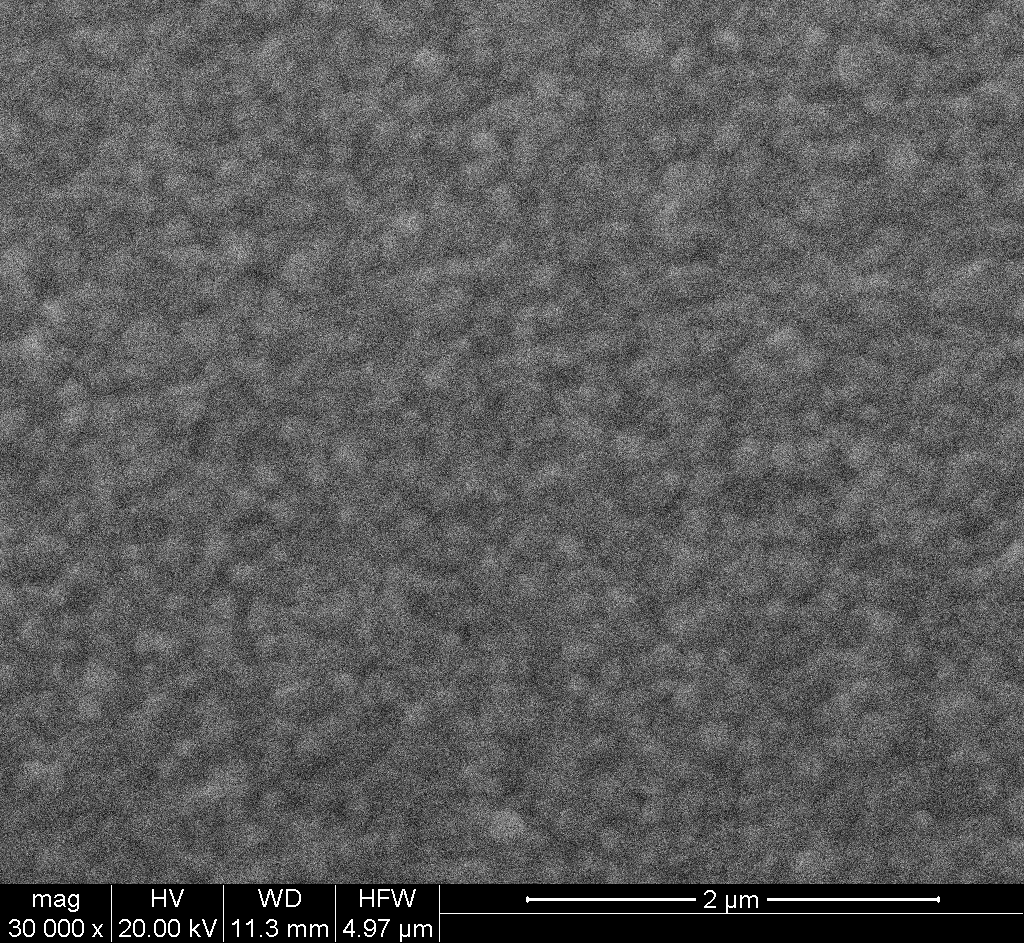
\includegraphics[width=1\textwidth]{esem-topview/ig87-c39-8000RPM-30k-hv-contrast.png}
				\subcaption{\SI{8000}{\rpm}, \SI{230}{\nm}}\label{fig:thickness-esem-topview-8000RPM}
			\end{subfigure}
			\qquad
			\begin{subfigure}[t]{0.51\textwidth}
				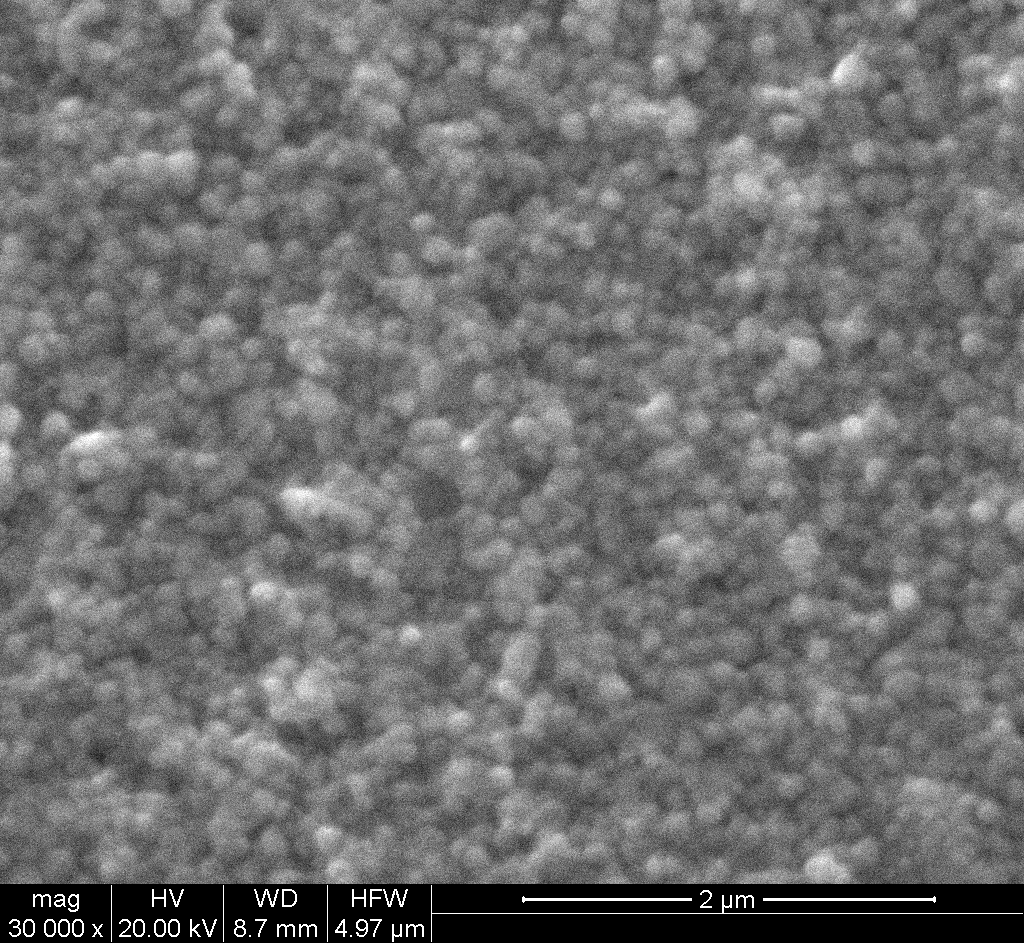
\includegraphics[width=1\textwidth]{esem-topview/ig87-b78-4100RPM-30k-hv-contrast.png}
				\subcaption{\SI{4100}{\rpm}, \SI{320}{\nm}}\label{fig:thickness-esem-topview-4100RPM}
			\end{subfigure}
			\bigskip
			
			\begin{subfigure}[t]{0.51\textwidth}
	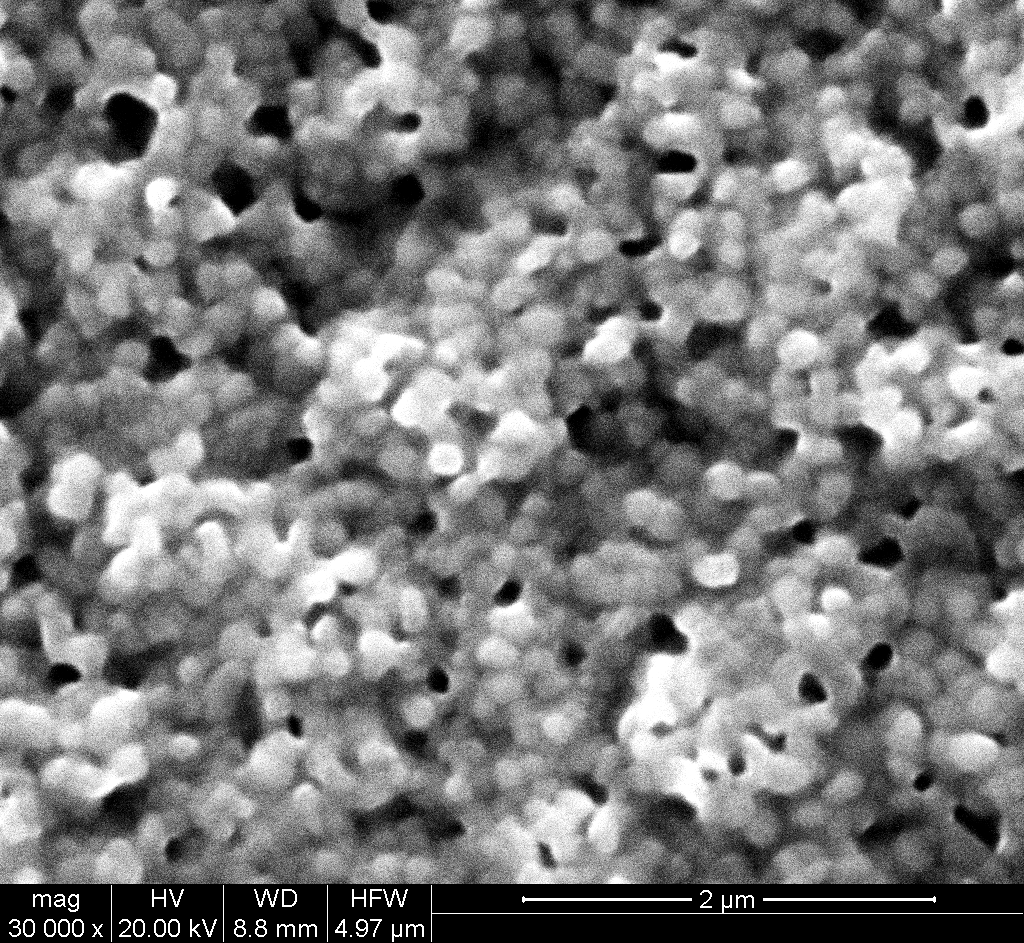
\includegraphics[width=1\textwidth]{esem-topview/ig87-c34-2000RPM-30k-hv-contrast.png}
	\subcaption{\SI{2000}{\rpm}, \SI{440}{\nm}}\label{fig:thickness-esem-topview-2000RPM}
\end{subfigure}
			
			\mycaption[Top view ESEM images of annealed perovskite layers with various thicknesses.]{The surface of a thin perovskite layer is studied using  FIJI/ImageJ \cite{Schindelin2012} on images of two different devices for each deposition condition (just one reported here for brevity). The average domain diameter and its standard deviation in parenthesis is \SI{182 \pm 25}{\nm} for the thin \SI{230}{\nm} perovskite layer in (\textbf{a}), \SI{190 \pm 34}{\nm} for the medium \SI{320}{\nm} perovskite layer in (\textbf{b}), \SI{189 \pm 23}{\nm} for the thick \SI{440}{\nm} perovskite layer in (\textbf{c}).}\label{fig:thickness-esem-topview}
		}
	}
\end{figure}


\begin{SCfigure}
	\centering
	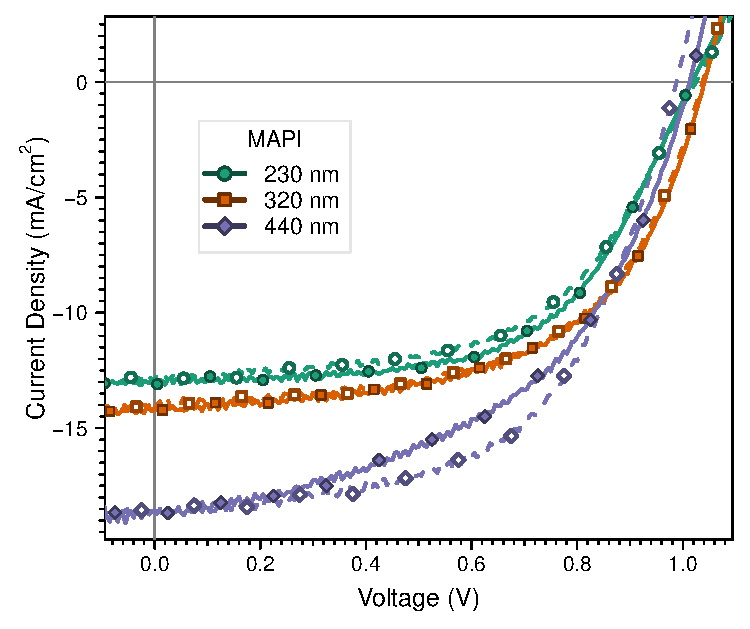
\includegraphics[width=0.7\textwidth]{jv_champions-mapi/mapi-IVs.pdf}
	\mycaption[Current-voltage sweeps for champion devices with different MAPI thicknesses.]{The solid line with filled markers represents the forward scan, while the dashed line with hollow markers represents the reverse scan.}\label{fig:jv_champions-mapi}
\end{SCfigure}





Figure 2 illustrates the current-voltage (J-V) characterization for three representative cells with different thicknesses of MAPI. It could be observed that increasing the MAPI thickness leads to an increase of the photocurrent and, thus, the overall solar cell efficiency (see Table 1). The fill factor (FF) is not heavily influenced by MAPI layer thickness increment so that we could assume that resistances are very similar as well as the interfaces with the respective electron transporting material (ETM) and the HTM (Figure S2). In order to ensure that the interfaces with the MAPI are similar using different thicknesses, ESEM imaging has been performed (See Figure S5); we have demonstrated that, even the roughness increase with the MAPI thicknesses, the grain size and distribution of the crystallites are almost identical.
Regarding the open circuit voltage (VOC), this value also barely changed with thickness. We have to highlight that both PCBM-C70 and PEDOT:PSS layers were likewise deposited to be the same for all the devices and in order to make a fair comparison. Despite this, it could be assumed that the charge losses and the overall resistance of the devices related to the contacts were very similar and, thus, the increase of the short-circuit current (JSC) can only be attributed to the increase of MAPI thickness.36 Using the same solar cells and in order to confirm these assertions, we performed Photo-Induced Differential Charging (PIDC), Photo-Induced Charge Extraction (PICE) and Photo-Induced Transient Photovoltage (PI-TPV) measurements as reported before.33, 37

Figure 2. Photocurrent vs voltage curves for MAPI solar cells with different MAPI thickness: 230 nm (1), 320 nm (2) and 440 nm (3).
PICE measurements were performed to measure the charge density of devices under working conditions (Figure S10a). There is a mandatory condition that gives reliability to this measurement: Decay from PICE has to be faster than voltage decay from PI-TPV transients.37 In our case, the PICE decay was slightly faster than PI-TPV; this ensures its correct interpretation (Figure S7). Alternatively, when the PICE and PI-TPV VOC decays lifetime were of the same order of magnitude, PIDC were measured giving a more representative calculated geometric capacitance (Cg) of 68, 65 and 41 nFcm-2 for devices 1, 2 and 3 respectively (Figure S10b) that are consistent with the ones obtained using PICE technique (Figure S10a). These results are, both using PICE and PIDC techniques, in perfect agreement to the parallel plate capacitor model where the Cg is inversely proportional to the distance between the two electrodes or, that is the same, the thickness of the device; this assumes that charges are stored, in open circuit conditions, at the contacts.
Moreover, in order to study the charge storage and recombination in the bulk of the device, close to 1 sun conditions, the Cg was subtracted from the total capacitance; the resulting chemical capacitance was integrated over voltage giving the charge density presumably stored at the bulk of the device at different light intensities.33, 38
PIDC measurements are depicted in Figure 3a. As can be seen, and despite the difference in thickness, the charge densities measured using PIDC in the three devices were very similar as well as the VOC, no shift in the charge distribution was observed that is in good agreement with the observed VOC from the J-V characterization. Furthermore, carrier recombination processes can be assessed using PI-TPV measurements; this technique allows the measurement of carriers’ lifetime under different light intensities at open circuit conditions. Figure 3b shows the PI-TPV measurement for devices 1, 2 and 3.


Figure 3. a) Charge density from PIDC (integrated chemical capacitance) at different voltages and b) Charge carrier lifetime at different charge density of devices 1 (230 nm), 2 (320 nm) and 3 (440 nm) using different thickness of MAPI.
As can be seen, the charge recombination follows same kinetics, in other words the three devices shown the same PI-TPV slope, and then no substantial differences could be considered. Thus, we have demonstrated that the increase of the JSC is directly related to the thickness of MAPI layer, with the VOC being equal for the three devices.



\section{Varying \glsentrytext{pcbm70} Thickness (\glsentryshort{etm} Layer)}

\cref{table:pcbm_thickness}

\begin{SCfigure}
	\centering
	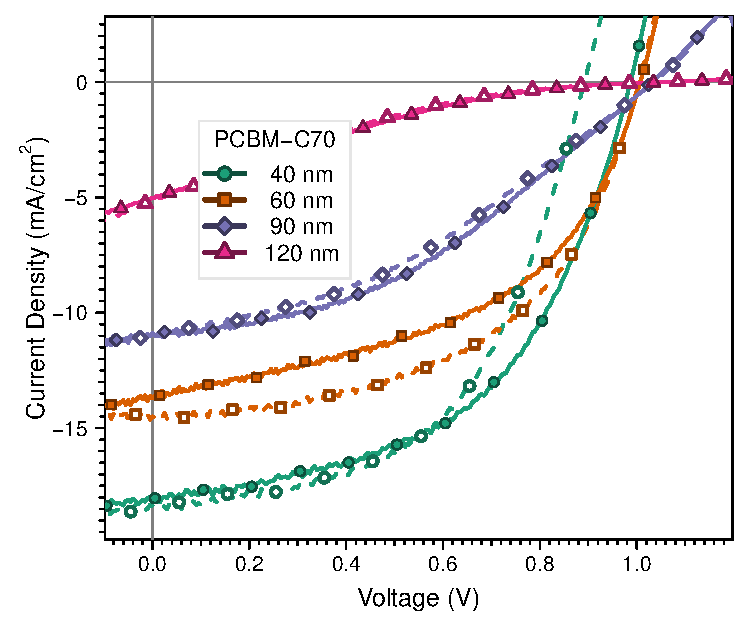
\includegraphics[width=0.7\textwidth]{jv_champions-pcbm/pcbm-IVs.pdf}
	\mycaption[Current-voltage sweeps for champion devices with different \glsentrytext{pcbm70} thicknesses.]{The solid line with filled markers represents the forward scan, while the dashed line with hollow markers represents the reverse scan.}\label{fig:jv_champions-pcbm}
\end{SCfigure}




s-shape curve when thick pcbm \cite{Wheeler2017} "build-up of space charge due to the restriction of carriers out of the device due to the slow mobility associated with the PCBM."


"The physical meaning of a small majority carrier surface-recombination velocity is an extraction barrier that would eventually lead to S-shaped light J-V curves. Experimentally, such S-shaped curves are not observed for the devices studied herein; however, S-shaped J-V curves could be observed in simulations when Smin is reduced and are discussed further in Supplemental Material [39]."
"Effect of reduced surface recombination velocityBothSmajandSminare predicted to cause S-shaped JV curves when very small, as seen infigure 7.  In the case ofSmaj,  as described by Wagenpfahlet al.,  a lowSmajrestrictsextraction of majority carriers out of the device.  This leads to a build-up of space chargein the device, lowering the VOC.  In the case of a lowSmin, restricting surface recombinationof  minority  carriers  causes  them  to  accumulate  at  the  electrode  around  open-circuit.   Inthe case of electrons at the anode, this causes the conduction band and the Fermi-level tocome closer together.  At open-circuit, by definition the Fermi-level is flat;  this forces theconduction band to bend down.  At voltages just less than VOC where charges still need tobe extracted, there is additional bulk recombination losses as electrons now have to diffuseagainst the electric field over a barrier to get collected at the cathode.  The simulated banddiagrams can be seen in figure 9."
"S-shaped JV curves as a consequence of a reduced minority surface-recombination velocity." \cite{Wheeler2015}

change in RC time due to increased PCBM layer resistance \cite{Wheeler2017}

importance of energy disorder in pcbm layer 10.1038/nenergy.2015.1





ETM layer was also tested, and in order to ensure good coverage in all devices the thickness of the MAPI devices were slightly reduced to 350 nm, resulting in smoother MAPI and allows the study of the PCBM-C70 with a wider range of thicknesses (see Figure S13). 
Figure 4 illustrates the measured J-V curves for four representative cells with different thicknesses of PCBM-C70: 40 nm (device 4), 60 nm (device 5), 90 nm (device 6) and 120 nm (device 7).

Figure 4. Photocurrent vs voltage curves for solar cells using 40 nm (4), 60 nm (5) 90 nm (6) and 120 nm (7) of PCBM-C70.
We could observe that device 4 presents the highest JSC of this set and a progressive decrease of the JSC with the increase in thickness of PCBM-C70, whereas the VOC show minor differences. The FF, on the contrary, drastically decrease as the ETM becomes thicker, that points out to an important resistance to transport, which is in agreement with the increase of the series resistances reflected in the J-V curves and the rise of the S-shape using 120 nm (7) of PCBM-C70.39-40 The mobility of the fullerene has been extensively reported41 being in the order of 10-3 cm2 V-1 s-1 witch is a low mobility value compared to MAPI44 or PEDOT:PSS45 layers, that becomes one of the main limitations for the inverted MAPI devices. Our results are in agreement with the previous publication of Seok et al.36
For device 7, photo-induced transient measurements have not been measured because of the extremely low performance. PIDC measurements for this set are shown in Figure 5a, in this case the geometric capacitance was calculated to be 57, 48 and 36 nF cm-2 for 40 nm (device 4), 60 nm (device 5) and 90 nm (device 6) thick PCBM-C70 layer respectively (Figure S11b). These differences observed in the Cg (low light intensities) are a direct indication that the system can be modeled as a parallel plate capacitor, as seen for different MAPI thicknesses. Thus, both layers, MAPI and PCBM-C70, are englobed in the semiconductor bulk between the two electrodes of the capacitor. We can determine that this system, far from 1 sun conditions, stores the charges at the Ag electrode. 
Additionally, and interestingly, we observed a shift on the measured charge distribution, from from PIDC for the thicker PCBM-C70 (Figure 5a). Huang and co-workers25 related the difference in the band tail of the charge distribution to changes in the energy disorder of the fullerene layer due to its lack of crystallinity and random molecular orientation and interaction with the perovskite. The measured exponential curve from PIDC clearly points out to this trend having the thickest devices the most disordered layer. That drove us to think that, close to 1 sun conditions, charges are mainly stored at the MAPI/PCBM-C70 interface.


Figure 5. a) Charge density from PIDC (integrated chemical capacitance) at different voltages and b) Charge carrier lifetime at their corresponding charge density of devices 4 (40 nm), 5 (60 nm) and 6 (90 nm) using different thickness of PCBM-C70.
Moreover, PICE was also measured for these devices, and we found that PICE decays were, in all cases, faster than PI-TPV decays. PICE of these devices are shown in the SI (Figure S11a) and a direct relationship is shown between total charges and the experimental JSC from J-V curves. It is clear that thicker PCBM-C70 layers impede the efficient collection of charges at the metal contact.





\section{Varying \glsentrytext{pedotpss} Thickness (\glsentryshort{htm} Layer)}

\begin{SCfigure}
	\centering
	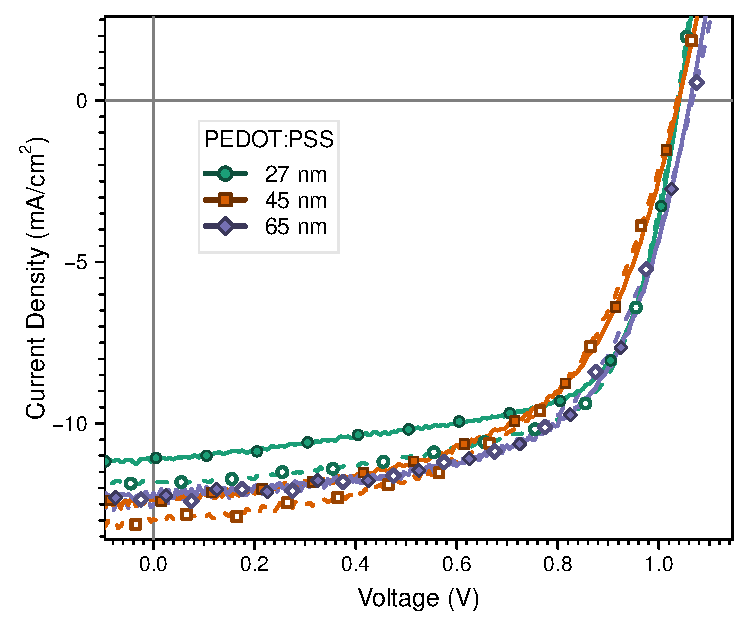
\includegraphics[width=0.7\textwidth]{jv_champions-pedotpss/pedotpss-IVs.pdf}
	\mycaption[Current-voltage sweeps for champion devices with different \glsentrytext{pedotpss} thicknesses.]{The solid line with filled markers represents the forward scan, while the dashed line with hollow markers represents the reverse scan.}\label{fig:jv_champions-pedotpss}
\end{SCfigure}

\cref{table:pedotpss_thickness}




Following same procedure, PEDOT:PSS layer was also studied using different thicknesses maintaining constant the MAPI (300 nm) and PCBM-C70 (40 nm) layers.
Figure 6 illustrates the J-V curves for a set of solar cells with different PEDOT:PSS layer thicknesses: 27 nm (device 8), 45 nm (device 9) and 65 nm (device 10). The JSC average (see Figure S4) reveals no evident variations due to the variation of PEDOT:PSS layer thickness as well as for the VOC and FF.

Figure 6. Photocurrent vs voltage curves for solar cells using 27 nm (8), 45 nm (9) and 65 nm (10) of PEDOT:PSS 


Figure 7. a) Charge density from PIDC (integrated chemical capacitance) at different voltages and b) Charge carrier lifetime at their corresponding charge density of devices 8 (27 nm), 9 (45 nm) and 10 (65 nm) using different thickness of PEDOT:PSS.
Furthermore, it is important to remark that the hole mobility of PEDOT:PSS is one order of magnitude higher (1·10-2 cm2V-1s-1)42 than the PCBM-C70 electron mobility, that means that this layer does not present significant resistance to transport of the holes. 
Therefore, the thickness does not become a limitation for the device operation. PICE, PIDC and PI-TPV were also performed to study the charge behavior changing PEDOT:PSS thickness. PICE and PIDC (Figure S12a and S12b) demonstrate in both cases very similar charge distribution, specially the Cg of the three devices seem to be identical around 50 nFcm-2 in PIDC and 58 nFcm-2 in PICE.
Furthermore, after subtracting the Cg from the total charge (Figure 7a), for the different PEDOT:PSS layer thicknesses the obtained charge density vs voltage curve is almost identical. In PI-TPV (Figure 7b) the charge lifetime were very similar for the three cases, device 9 presents quite slower charge recombination rates at 1 sun conditions, but the differences were not as substantial as to be considered a direct consequence of the difference in PEDOT:PSS layer thickness. The conclusion that can be extracted from these results is that PEDOT:PSS thickness does not affect the charge distribution, indicating that holes are mainly stored at the ITO/PEDOT:PSS interface, in other words, PEDOT:PSS does not play any role in the charge accumulation, in contrast to the electrons that are seemed to be stored at PCBM-C70/MAPI interface.
In conclusion, we have fabricated hybrid perovskite solar cells using inverted structure achieving efficiencies up to 10 % under standard solar simulation conditions. The maximum efficiency was obtained through the optimization of the thickness of selective contact layer for electrons (PCBM-C70) and, on the other hand, the optimization of the photoactive perovskite layer. The optimization was carried out analyzing the carrier accumulation at different light bias and the carrier lifetime between different solar cells. We observed in all cases an extended linear relationship between the measured charge and the light bias for values from 0 V (dark conditions) to 0.8 V. This implies that, under open circuit conditions and far from 1 sun conditions, the charges are mainly accumulated at the selective contact electrodes. An exponential increase, which results from the charge accumulation at the photoactive layer, appeared at potentials close to 1 sun simulated conditions (0.8-1.1 V).
Moreover, for devices with different MAPI layer thickness all the charge distribution and recombination rates were very similar indicating that the device performance was mainly limited by the organic contacts, PEDOT:PSS and PCBM-C70. In these devices the increase of the measured JSC can be directly related to the increase of the MAPI layer thickness. While modifying the thickness of PCBM-C70 we found an important impact on performance as well as a different charge distribution and recombination. The device with the thinnest PCBM-C70 layer presented the highest JSC and FF due to its low resistance to transport. In addition, the PIDC controversially showed higher charge densities using thicker layers of PCBM-C70 that means greater amount of charges stored at the bulk, however the recombination (at 1 sun conditions) becomes faster due to the mentioned transport losses and the extraction of these charges becomes less efficient. At this point, the geometric capacitance has been strongly influenced by both MAPI and PCBM-C70 thickness layer variation; this is an indication that the charges are mainly stored at the PCBM-C70/MAPI interface.
Finally, it was demonstrated that modifying PEDOT:PSS layer do not affect the final device performance, and PIDC, PICE and PI-TPV measurements present no evaluable differences. This points out that, due to the great hole mobility of the PEDOT:PSS layer, this organic layer does not limits the performance of the devices, and the holes would be mainly stored at the ITO /PEDOT:PSS interface and thus the thickness of the PEDOT:PSS do not play any role in the storage but in the extraction.






\section{Conclusions}
\section{Critical Assessment}




